\documentclass{article}

\usepackage{geometry}
\usepackage{amsmath}
\usepackage{graphicx}
\usepackage{listings}
\usepackage{hyperref}
\usepackage{multicol}
\usepackage{fancyhdr}
\pagestyle{fancy}
\hypersetup{ colorlinks=true, linkcolor=black, filecolor=magenta, urlcolor=cyan}
\geometry{ a4paper, total={170mm,257mm}, top=20mm, right=20mm, bottom=20mm, left=20mm}
\setlength{\parindent}{0pt}
\setlength{\parskip}{1em}
\renewcommand{\headrulewidth}{0pt}
\lhead{Competitive Programming - Arkavidia V}
\fancyfoot[CE,CO]{\thepage}

\begin{document}

\begin{center}
    \section*{E. Eksplorasi Pola} % ganti judul soal

    \begin{tabular}{ | c c | }
        \hline
        Batas Waktu  & 1s \\    % jangan lupa ganti time limit
        Batas Memori & 64MB \\  % jangan lupa ganti memory limit
        \hline
    \end{tabular}
\end{center}

\subsection*{Deskripsi}

Suatu hari, Arvy sedang belajar bermain rubik berukuran $N$x$N$x$N$.
Ia merepresentasikan jenis putaran yang ia lakukan pada rubik dengan perintah $X_1,X_1',X_2,X_2',\dots,X_N,X_N',Y_1,Y_1',Y_2,Y_2',\dots,Y_N,Y_N',Z_1,Z_1',Z_2,Z_2',\dots,Z_N,Z_N'$ dengan arah rotasi seperti pada gambar. 
Sebagai contoh, $X_1$ akan memutar rubik searah dengan panah warna hijau, $Y_2'$ akan memutar rubik searah dengan panah warna ungu, $Z_2$ akan memutar rubik searah dengan panah warna hitam. 
Perintah $Z_2,Z_1'$ akan mengubah rubik pada bagian kiri menjadi rubik pada bagian kanan.

\begin{center}
    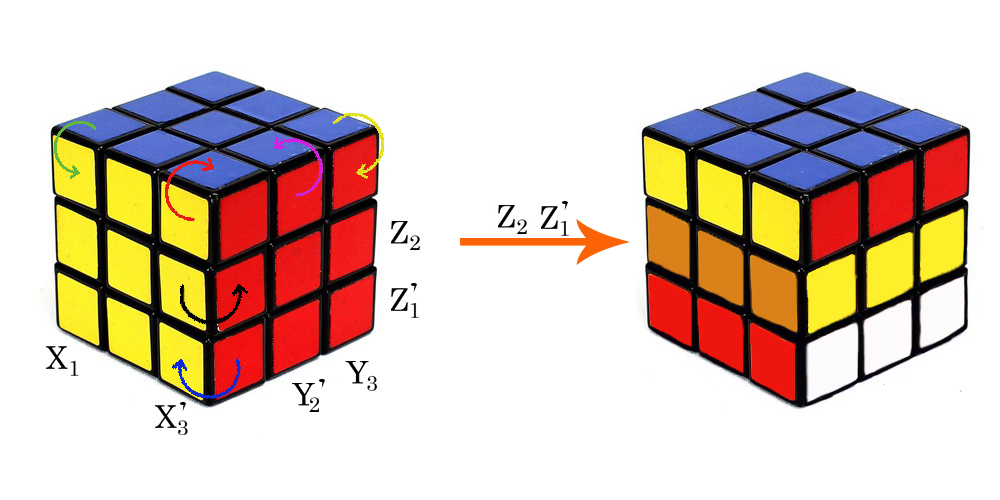
\includegraphics[width=350px]{rubic}
\end{center}
Ia menyadari ada hal yang unik dari putaran ini.
Pertama, Arvy menuliskan beberapa perintah pemutaran rubik.
Kemudian, ia melakukan perintah yang ia tulis tadi berulang-ulang dan ternyata rubik dapat kembali ke pola semula.
Arvy penasaran berapa kali ia harus mengulang perintah yang sama agar rubik kembali ke pola semula.

\subsection*{Format Masukan}

Baris pertama terdiri dari satu bilangan bulat positif $T$ ($1 \leq T \leq 100.000$), menyatakan banyaknya kasus uji.
TBD

\subsection*{Format Keluaran}

Untuk tiap kasus uji, tuliskan bilangan N yang menyatakan banyaknya pengulangan perintah yang sama agar rubik kembali ke pola semula.
\\

\begin{multicols}{2}
\subsection*{Contoh Masukan 1}
\begin{lstlisting}
TBD
\end{lstlisting}
\columnbreak
\subsection*{Contoh Keluaran 1}
\begin{lstlisting}
TBD
\end{lstlisting}
\vfill
\null
\end{multicols}

\begin{multicols}{2}
\subsection*{Contoh Masukan 2}
\begin{lstlisting}
TBD
\end{lstlisting}
\columnbreak
\subsection*{Contoh Keluaran 2}
\begin{lstlisting}
TBD
\end{lstlisting}
\vfill
\null
\end{multicols}

% \subsection*{Penjelasan}
% Jika dibutuhkan, tambahkan penjelasan di sini

\pagebreak

\end{document}